%%%%%%%%%%%%%%%%%%%%%%%%%%%%%%%%%%%%%%%%%
% Short Sectioned Assignment
% LaTeX Template
% Version 1.0 (5/5/12)
%`
% This template has been downloaded from:
% http://www.LaTeXTemplates.com
%
% Original author:
% Frits Wenneker (http://www.howtotex.com)
%
% License:
% CC BY-NC-SA 3.0 (http://creativecommons.org/licenses/by-nc-sa/3.0/)
%
%%%%%%%%%%%%%%%%%%%%%%%%%%%%%%%%%%%%%%%%%

%----------------------------------------------------------------------------------------
%	PACKAGES AND OTHER DOCUMENT CONFIGURATIONS
%----------------------------------------------------------------------------------------

\documentclass{article}

\usepackage[T1]{fontenc} % Use 8-bit encoding that has 256 glyphs
%\usepackage{fourier} % Use the Adobe Utopia font for the document - comment this line to return to the LaTeX default
\usepackage[english]{babel} % English language/hyphenation
\usepackage{amsmath,amsfonts,amsthm, amssymb} % Math packages
\usepackage{sectsty} % Allows customizing section commands
\usepackage{tikz-cd} % Allows for commutative diagrams
\usepackage{tikz}
\usetikzlibrary{graphs, graphs.standard, quotes}% quotes library is for the [""] edges
\usepackage[]{enumerate} %Changing enumerate environment
\usepackage{mathrsfs} %fonts?
\usepackage{cancel} % for pretty slashes
\usepackage{graphicx}
\usepackage{float}

%%%% The following is the format I'm using for boxes %%%%
%	
%	
%\fbox{	
%\begin{minipage}{.9\textwidth}
%	\textbf{Wilson's Algorithm:} 
%		\begin{enumerate}
%		\item Pick a root vertex $r$, not necessarily uniformly from $G$, and set $T_0 = \{r\}$. 
%		\item Repeat the following:
%		\begin{enumerate}
%			\item Select a random vertex $v_i$ uniformly from vertices not in $T_i$.
%			\item Perform a \textit{loop-erased random walk} (LERW) in $G$ until we find a path $P_i$ whose first vertex is $v_i$ and whose last vertex is in $T_i$. 
%			\item Set $T_{i+1} = T_i \cup P_i$.
%			\item Do until the vertices of $T_k$ span the vertices of $G$.
%		\end{enumerate}
%	\end{enumerate}
%\end{minipage}
%}\\

%% example graph %%
%\begin{tikzpicture}[node distance = {1.0cm and 1.5cm}, v/.style = {draw, circle}]
%\graph[nodes={circle, draw}, grow right=2.25cm, branch down=1.75cm]{
%	A -- ["1"] C -- ["3"] E,
%	B -- ["1",swap] D -- ["4",swap] F,
%	B -- ["2"] A,
%	C -- ["2"] {D,B},
%	D -- ["3",swap] E -- ["1"] F
%};
%\end{tikzpicture}


\begin{document}
	
	\title{Combinatorics and Computation Notes}
	\author{Marissa Masden}
	\date{11/8/2019}
	\maketitle
	
	\section{The Perfect Matching Problem: Dimer Model}
	
	We will discuss the \textit{perfect matching problem} on connected, \textit{planar, bipartite} graphs. To begin, we must understand what each of these terms mean. \\
		
		
	\subsection{Planar Graphs}
	\fbox{	
		\begin{minipage}{.9\textwidth}
			
			A graph $G$ is called \textbf{planar} if, intuitively, $G$ can be drawn in the plane so that no two of its edges cross. More formally, there is an embedding of $G$, as a simplicial complex, in the plane.
			
		\end{minipage}
	}\\ \\
	
	Note, in particular, that $K_4$, the complete graph on $4$ vertices, is planar, even though the immediate way one might draw $K_4$ does not immediately appear planar:	
	\begin{figure}[H]
		\begin{center}
			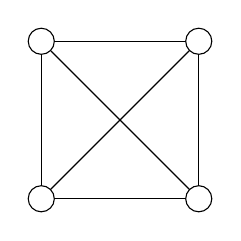
\begin{tikzpicture}[node distance = {1.0cm and 1.5cm}, v/.style = {draw, circle}]
			\graph[nodes={circle, draw}, grow right=2cm, branch down=2cm, empty nodes]{
				1 -- 2,
				3 -- 4,
				1 -- 3,
				1 -- 4,
				3 -- 2,
				4 -- 2			
			};
			\end{tikzpicture} \hspace{0cm} 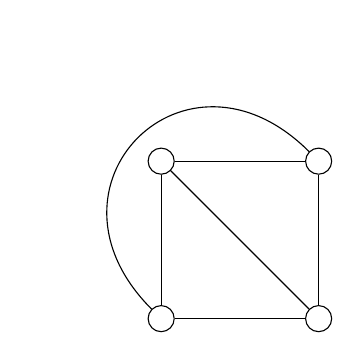
\begin{tikzpicture}[node distance = {1.0cm and 1.5cm}, v/.style = {draw, circle}]
			\graph[nodes={circle, draw}, grow right=2cm, branch down=2cm, empty nodes]{
				1 -- 2,
				3 -- 4,
				1 -- 3,
				1 -- 4,
				3 -- [bend left=90, looseness=2] 2,
				4 -- 2			
			};
			\end{tikzpicture} \hspace{1 cm}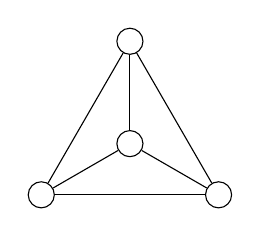
\begin{tikzpicture}[node distance = {1.0cm and 1.5cm}, v/.style = {draw, circle}]
			\graph[nodes={circle, draw}, grow right=2cm, branch down=2cm, empty nodes]
			{	
				subgraph C_n [n=1, name=inner, clockwise, radius=0 cm] --
				subgraph C_n [n=3,name=outer, clockwise,radius=1.3cm]
			};
			\end{tikzpicture} 
		\end{center}
		\caption{$K_4$, and two planar embeddings.} \label{fig:K4}
	\end{figure}
	
	For a fixed embedding of a planar graph, the graph partitions the plane into several open regions: one infinite region and many finite regions. These regions are called \textbf{faces}, for a reason that may become more obvious below. As seen in the previous example, the number of ``sides'' or ``edges'' of different faces may differ based on the choice of embedding of $G$. However, we do observe the following relationship which applies to any embedding of $G$, which should be familiar:\\
	
	\fbox{	
		\begin{minipage}{.9\textwidth}
			\textbf{Euler Characteristic of a Planar Graph}\\
			
			For any embedding of a planar graph $G=(V,E)$ which divides the plane into $|F|$ faces, 
			$$|V| - |E| + |F| = 2 $$
			
		\end{minipage}
	}\\ \\
	
	Euler originally proved this relationship for faces, vertices, and edges of polyhedra whose surfaces are topologically equivalent to the sphere $S^2$. We can understand why this same relationship appears for planar graphs by compactifying the single infinite face, creating an embedding of the graph in the sphere $S^2$. Alternately, the relationship may be proven by induction on $|V|+|E|$. 
	
	\subsection{Bipartite Graphs}
	
		\fbox{	
		\begin{minipage}{.9\textwidth}
			\textbf{Bipartite Graph}\\
			
			A graph $G = (V,E)$ is called \textbf{bipartite} if we may write $V = V_\circ \sqcup V_\bullet$ (think $V_{white} \sqcup V_{black}$) so that if $(u,v) \in E$, then either: 
			\begin{enumerate}\setlength\itemsep{-.2em}
				\item $u \in V_\circ$ and $v \in V_\bullet$, or 
				\item $v \in V_\circ$ and $u \in V_\bullet$ 
			\end{enumerate}
		
			Equivalently, $G$ is $2$-colorable.
		\end{minipage}
	}\\ \\

	For example, any even cycle graph is bipartite (two-colorable), whereas any odd cycle graph is not: 
	\begin{figure}[H]
	\begin{center}
			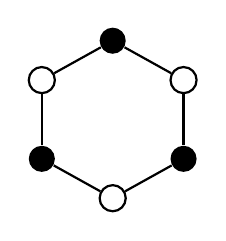
\begin{tikzpicture}[scale=.5]
			\node[shape=circle,text=white,fill=black] (A) at (0,2) {};% {$1$};
			\node[shape=circle,draw=black, thick] (B) at (1.8,1) {};% {$\bar{1}$};
			\node[shape=circle,text=white,fill=black] (C) at (1.8,-1) {};%{$2$};
			\node[shape=circle,draw=black,thick] (D) at (0,-2) {};% {$\bar{2}$};
			\node[shape=circle,text=white,fill=black] (E) at (-1.8,-1) {};% {$3$};
			\node[shape=circle, draw=black,thick] (F) at (-1.8,1) {};% {$\bar{3}$};
			
			\path [-, thick, black] (A) edge (B);
			\path [-, thick, black] (B) edge (C);
			\path [-, thick, black] (C) edge (D);
			\path [-, thick, black] (D) edge (E);
			\path [-, thick, black] (E) edge (F);
			\path [-, thick, black] (F) edge (A);
		\end{tikzpicture}
	\end{center}
		\caption{$C_6$ with $V_\circ$ colored white and $V_\bullet$ colored black.}
	\end{figure}
	
	 Determining if a graph is bipartite is straightforward: Start at one node and color it your favorite color (which is obviously black). Then proceed to each connected node and color it your second favorite color (white). Continue by proceeding to nodes which are connected to colored nodes, and coloring them either black or white so that no two connected nodes have the same color. If this becomes impossible, the graph is not bipartite. 
	
	
	\subsection{The Dimer Model} 
	
	\fbox{	
		\begin{minipage}{.9\textwidth}
			\textbf{Perfect Matching}\\ \\
			Let $G = (V,E)$ be a planar bipartite graph. A \textbf{perfect matching} on $G$ is a subgraph $M = (V, \tilde{E})$ such that every vertex in $M$ has degree $1$. 
		\end{minipage}
	}\\ \\

	We could equivalently call $M$ a \textbf{dimer cover} of $G$; this term arises from statistical mechanics, where a dimer refers to a polymer formed of only two monomers, that is, a chain with only two links.
	
	Below we see one of many possible perfect matchings on a grid graph: 
	
	\begin{figure}[H]
		
	\begin{center}
		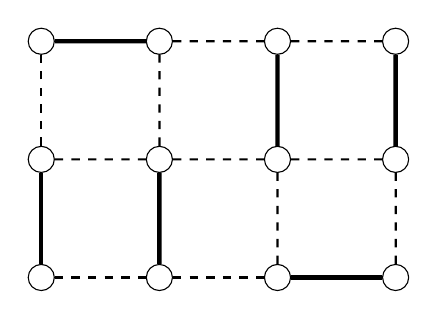
\begin{tikzpicture}[scale=1.5]
		\node[shape=circle,text=white,draw=black] (A) at (0,0){};
		\node[shape=circle,text=white,draw=black] (B) at (1,0){};
		\node[shape=circle,text=white,draw=black] (C) at (2,0){};
		\node[shape=circle,text=white,draw=black] (D) at (3,0){};
		\node[shape=circle,text=white,draw=black] (E) at (0,1){};
		\node[shape=circle,text=white,draw=black] (F) at (1,1){};
		\node[shape=circle,text=white,draw=black] (G) at (2,1){};
		\node[shape=circle,text=white,draw=black] (H) at (3,1){};
		\node[shape=circle,text=white,draw=black] (I) at (0,2){};
		\node[shape=circle,text=white,draw=black] (J) at (1,2){};
		\node[shape=circle,text=white,draw=black] (K) at (2,2){};
		\node[shape=circle,text=white,draw=black] (L) at (3,2){};		

		
		\path [-, dashed, thick, black] (A) edge (B);
		\path [-, dashed, thick, black] (B) edge (C);
		\path [-, ultra thick, black] (C) edge (D);
		\path [-, dashed, thick, black] (E) edge (F);
		\path [-, dashed, thick, black] (F) edge (G);
		\path [-, dashed, thick, black] (G) edge (H);
		\path [-, ultra thick, black] (I) edge (J);
		\path [-, dashed, thick, black] (J) edge (K);
		\path [-, dashed, thick, black] (K) edge (L);
		
		\path [-, ultra thick, black] (A) edge (E);
		\path [-, ultra thick, black] (B) edge (F);
		\path [-, dashed, thick, black] (C) edge (G);
		\path [-, dashed, thick, black] (D) edge (H);
		\path [-, dashed, thick, black] (E) edge (I);
		\path [-, dashed, thick, black] (F) edge (J);
		\path [-, ultra thick, black] (G) edge (K);
		\path [-, ultra thick, black] (H) edge (L);
		\end{tikzpicture}
	\end{center}
		
		
		\caption{A perfect matching on $3 \times 4$ grid graph}
	\end{figure}

	We wish to construct a probability measure on all perfect matchings on a graph. It is constructed as follows: Let $w: E \rightarrow \mathbb{R}_{\geq 0}$ be a weight function on $E$ and define\footnote{If, for some reason, you wish to have weights behave additively, take exponents.} $$w(M) = \prod_{e \in \tilde{E}} w(e) $$
	
	 Then we have a total measure $$Z(G) = \sum_{M \text{ perfect}} w(M),$$ which is often called the \textbf{partition function} of $G$, again arising from statistical mechanics jargon. This allows us to construct a probability measure on perfect matchings: \\
		
		\fbox{	
		\begin{minipage}{.9\textwidth}
			\textbf{Dimer Model} \\ \\
			The \textbf{dimer model} is the probability measure on perfect matchings $M$  of $G$ where: 
			
			$$\mathbb{P}(M) \propto w(M) $$
			or equivalently 
			
			$$ \mathbb{P}(M) = \frac{w(M)}{Z(G)}$$ 
		\end{minipage}
	}\\ \\

The simplest case of the dimer model occurs when we set $w \equiv 1$, that is, all edges are weighted equally, and consequently so are the perfect matchings. In this case, $Z(G)$ is equal to simply the number of perfect matchings.

	
	
	
	\subsection{Counting Perfect Matchings}
	
	
	Throughout this section, we will let $G=(V,W)$ be a connected, planar, bipartite graph with a fixed embedding in the plane, and set $w \equiv 1$. Computing the number of perfect matchings is thus equivalent to computing $Z(G)$. Some graphs have very few perfect matchings;  for example, $C_{2k}$ has only two perfect matchings: \\
	
	\begin{figure}[H]
		
		\begin{minipage}{.45\textwidth}
			\begin{center}

					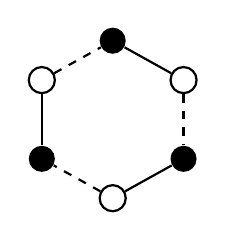
\begin{tikzpicture}[scale=.5]
					\node[shape=circle,text=white,fill=black] (A) at (0,2) {};% {$1$};
					\node[shape=circle,draw=black, thick] (B) at (1.8,1){};% {$\bar{1}$};
					\node[shape=circle,text=white,fill=black] (C) at (1.8,-1){};% {$2$};
					\node[shape=circle,draw=black,thick] (D) at (0,-2){};% {$\bar{2}$};
					\node[shape=circle,text=white,fill=black] (E) at (-1.8,-1){};% {$3$};
					\node[shape=circle, draw=black,thick] (F) at (-1.8,1){};% {$\bar{3}$};
					
					\path [-, thick, black] (A) edge (B);
					\path [-, dashed, thick, black] (B) edge (C);
					\path [-, thick, black] (C) edge (D);
					\path [-, dashed, thick, black] (D) edge (E);
					\path [-, thick, black] (E) edge (F);
					\path [-, dashed, thick, black] (F) edge (A);
					\end{tikzpicture}
			\end{center}

		\end{minipage}\begin{minipage}{.45\textwidth}
			\begin{center}
			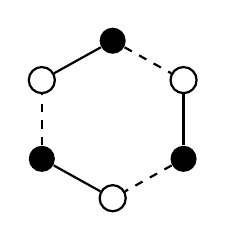
\begin{tikzpicture}[scale=.5]
			\node[shape=circle,text=white,fill=black] (A) at (0,2){};% {$1$};
			\node[shape=circle,draw=black, thick] (B) at (1.8,1){};% {$\bar{1}$};
			\node[shape=circle,text=white,fill=black] (C) at (1.8,-1){};% {$2$};
			\node[shape=circle,draw=black,thick] (D) at (0,-2){};% {$\bar{2}$};
			\node[shape=circle,text=white,fill=black] (E) at (-1.8,-1){};% {$3$};
			\node[shape=circle, draw=black,thick] (F) at (-1.8,1){};% {$\bar{3}$};
			
			\path [-, dashed, thick, black] (A) edge (B);
			\path [-, thick, black] (B) edge (C);
			\path [-, dashed, thick, black] (C) edge (D);
			\path [-, thick, black] (D) edge (E);
			\path [-, dashed, thick, black] (E) edge (F);
			\path [-, thick, black] (F) edge (A);
			\end{tikzpicture}
		\end{center}
	\end{minipage}
		\caption{The only two perfect matchings on $C_6$}
	\end{figure}

	As is the case for many calculations in this class, we will find that it is possible to compute the number of perfect matchings on a graph by taking the determinant of a matrix. First, note that because $G$ is bipartite, we may write its adjacency matrix  $A$ in blocks as follows, ordering the vertex set of $G$ by placing the vertices in $V_\bullet$ before those in $V_\circ$: 
	
	$$ A = \left[
	\begin{array}{c|c}
		0 & B \\[.2em]
		\hline 
		B^T & 0		
	\end{array}
	\right] $$
	
	Observe that the rows of $B$ are indexed by vertices $ 1, 2, ..., n \in V_\bullet$ and the columns are indexed by vertices $\bar{1}, \bar{2}, ..., \bar{m} \in V_\circ$. Thus $B$ is a matrix with a $1$ in entry $ij$ if vertex $i$ is connected to vertex $\bar{j}$, and a $0$ otherwise. We often call $B$ the \textbf{bipartite adjacency matrix} of a graph. Note that for a general bipartite graph we do not need $B$ to be square, but in order for a perfect matching to exist this is necessary. We will thus work under the assumption $m=n$. We could also weight the entries of $B$ by $w(e)$ as mentioned in the previous subsection.\\ 
	
	The next fact we will observe is that $$\det B = \sum_{M \text{ perfect}} \varepsilon(M) w(M),$$ where $\varepsilon(M) = -1$ or $1$ depending on each matching in a nonobvious way. This arises from the permutation expansion of a determinant. Recall that for any matrix: 
	
	$$ \det [a_{ij}] = \sum_{\sigma \in S_n} \text{sgn}(\sigma)a_{1\sigma_1} a_{2\sigma_2} .. a_{n\sigma_n} $$ 
	
	For our matrix $B$, we claim that an entry in the above sum corresponds to a hypothetical matching, and is either $0$ or $\pm w(M)$ depending on whether that matching exists. To see this, we represent $\sigma$ in two-line notation. Each column gives us a matching between $1, 2, ..., n \in V_\bullet$ and $\bar{1} , ... , \bar{n} \in V_\circ$. For example, the permutation $\sigma = (132)$ in $S_3$ corresponds with a perfect matching in the $C_6$ graph:
	
	\begin{figure}[H]
		\begin{minipage}{.45\textwidth}
				$$\sigma = \begin{pmatrix}
			1 & 2 & 3 \\ 
			\bar{3} & \bar{1} & \bar{2}
			\end{pmatrix} $$
		\end{minipage}\hspace{1 cm}		\begin{minipage}{.45\textwidth}
			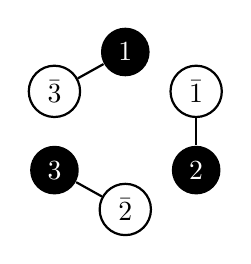
\begin{tikzpicture}[scale=.5]
			\node[shape=circle,text=white,fill=black] (A) at (0,2)  {$1$};
			\node[shape=circle,draw=black, thick] (B) at (1.8,1) {$\bar{1}$};
			\node[shape=circle,text=white,fill=black] (C) at (1.8,-1){$2$};
			\node[shape=circle,draw=black,thick] (D) at (0,-2) {$\bar{2}$};
			\node[shape=circle,text=white,fill=black] (E) at (-1.8,-1){$3$};
			\node[shape=circle, draw=black,thick] (F) at (-1.8,1) {$\bar{3}$};
			
			%\path [-, thick, black] (A) edge (B);
			\path [-, thick, black] (B) edge (C);
			%\path [-, thick, black] (C) edge (D);
			\path [-, thick, black] (D) edge (E);
			%\path [-, thick, black] (E) edge (F);
			\path [-, thick, black] (F) edge (A);
			\end{tikzpicture}
		\end{minipage}
		
		
		\caption{A permutation and corresponding perfect matching}
	\end{figure}
	
	Since  $a_{i \sigma_i}$ is $0$ if an edge does not exist, and $w(i\sigma_i)$ otherwise, each term of the permutation expansion gives $0$ if there are missing edges in a hypothetical matching, or $w(M)$ if all requisite edges are present. \\ 
	
	We continue by computing the determinant of the bipartite matrix of $C_6$ via permutation expansion:
	
	$$B = \begin{bmatrix}
	1& 0 & 1 \\ 
	1 & 1 & 0 \\ 
	0 & 1 & 1
	\end{bmatrix} \qquad \det B = (1\cdot 1 \cdot 1) \text{sgn}(id)  + (1\cdot 1 \cdot 1) \text{sgn}(123) = 2 $$

	It just so happened that in this case, $\det B = Z(G)$. However, this only happened because sgn$(\sigma)= 1$ for each permutation corresponding to a perfect matching. This does not happen for $C_4$: 
	
	\begin{figure}[H]
		\begin{minipage}{.3\textwidth}
			\begin{center}
				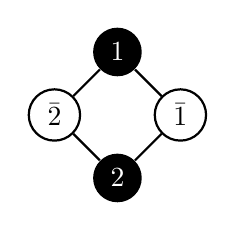
\begin{tikzpicture}[scale=.4]
				\node[shape=circle,text=white,fill=black] (A) at (0,2)  {$1$};
				\node[shape=circle,draw=black, thick] (B) at (2,0) {$\bar{1}$};
				\node[shape=circle,text=white,fill=black] (C) at (0,-2){$2$};
				\node[shape=circle,draw=black,thick] (D) at (-2,0) {$\bar{2}$};
				
				
				\path [-, thick, black] (A) edge (B);
				\path [-, thick, black] (B) edge (C);
				\path [-, thick, black] (C) edge (D);
				\path [-, thick, black] (D) edge (A);
				\end{tikzpicture}
			\end{center}
		\end{minipage}\hspace{.2 cm}\begin{minipage}{.3\textwidth}
		$$ B = \begin{bmatrix}
		1 & 1 \\ 1 & 1
		\end{bmatrix}$$
	\end{minipage}\hspace{.2 cm}\begin{minipage}{.3 \textwidth}
	\begin{align*}
		\det B &= (1\cdot 1 ) \text{sgn}(id)\\ & \quad + (1 \cdot 1) \text{sgn}(21) \\&= 1-1\\ &= 0
	\end{align*}
\end{minipage}
	\end{figure}
	
	However, the failure of this determinant to calculate the number of perfect matchings can be remedied by constructing a new matrix $K$,simply by putting a negative sign on some entries of $B$: 
	
	$$K = \begin{bmatrix}
	-1 & 1 \\ 
	1 & 1
	\end{bmatrix}, \qquad \det K = 2$$
	
	It is a a nontrivial theorem that this approach can, in fact, work in all cases:\\ 

			\fbox{	
		\begin{minipage}{.9\textwidth}
			\textbf{Theorem (Kastelyn, 1961)} \\ \\
			If $B= [w(ij)]$ is the bipartite adjacency matrix associated with a biparatite graph, then there is a choice of signs $\sigma: E \rightarrow \{ \pm 1 \}$ and a matrix $K$ so that
			
			$$K = [w(ij) \sigma(ij)]_{\substack{i \in V_\bullet \\  j \in V_\circ}} $$ 
			
			and $\det K = \pm Z(G)$		
				 
		\end{minipage}
			}\\ \\
		
		We call $K$ the \textbf{Kastelyn Matrix} associated with a bipartite graph. It is possible to construct $\sigma$ by arranging for each face $F = \{ e_1, ..., e_{2k} \}$ to satisfy the following \textbf{multiplicative edge condition}: 
		
		$$ \prod_{i=1}^{2k} \sigma(e_i) = \begin{cases}
		1 & \text{$k$ odd}\\
		-1 & \text{$k$ even}
		\end{cases} $$
		
		The intuition behind this is that the following pair of perfect matchings should correspond to equal values in the permutation expansion, but they correspond to permutations with opposite signs, and this happens precisely when you have a cycle of length $4k$:
		
\begin{figure}[H]
	\begin{minipage}{.45\textwidth}
		\begin{center}
				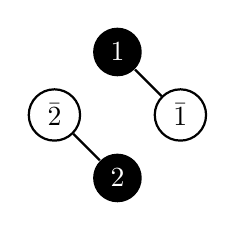
\begin{tikzpicture}[scale=.4]
			\node[shape=circle,text=white,fill=black] (A) at (0,2)  {$1$};
			\node[shape=circle,draw=black, thick] (B) at (2,0) {$\bar{1}$};
			\node[shape=circle,text=white,fill=black] (C) at (0,-2){$2$};
			\node[shape=circle,draw=black,thick] (D) at (-2,0) {$\bar{2}$};
			
			
			\path [-, thick, black] (A) edge (B);
			%\path [-, thick, black] (B) edge (C);
			\path [-, thick, black] (C) edge (D);
			%\path [-, thick, black] (D) edge (A);
			\end{tikzpicture}
		\end{center}
		
	\end{minipage}\begin{minipage}{.45\textwidth}
		\begin{center}
				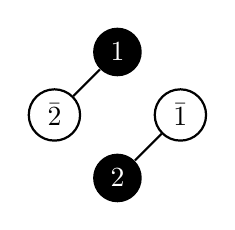
\begin{tikzpicture}[scale=.4]
			\node[shape=circle,text=white,fill=black] (A) at (0,2)  {$1$};
			\node[shape=circle,draw=black, thick] (B) at (2,0) {$\bar{1}$};
			\node[shape=circle,text=white,fill=black] (C) at (0,-2){$2$};
			\node[shape=circle,draw=black,thick] (D) at (-2,0) {$\bar{2}$};
			
			
			%\path [-, thick, black] (A) edge (B);
			\path [-, thick, black] (B) edge (C);
			%\path [-, thick, black] (C) edge (D);
			\path [-, thick, black] (D) edge (A);
			\end{tikzpicture}
		\end{center}
	\end{minipage}
\caption{Two perfect matchings in $4k$-cycles whose corresponding permutations have opposite signs.}
\end{figure}
		
		An algorithm to check each face one at a time systematically and change at most one edge in each face is as follows: \\ 
		
		
			\fbox{	
			\begin{minipage}{.9\textwidth}
				\textbf{Algorithm for assigning signs to edges:} \\ \\
				Fix an embedding of $G$ in the plane, so $G = (V,E,F)$. Then construct the \textbf{dual graph} $G^*$ of $G$, which has a vertex for every face, and edges connecting each adjacent face in $F$ across each edge in $E$ they share. In particular, every edge $e \in E$ is in bijection with edges $e^*$ in of $G^*$, since adjacent faces share edges. \\
				
				Find a spanning tree $T$ of  $G^*$ and select one node to be the root.\\
				
				Start changing signs by considering a face $f$ corresponding to an outermost leaf $f^*$ of $T$. Check to see if $f$ satisfies the multiplicative edge condition. If necessary, change the sign of one edge of $f$: the edge $e$ which corresponds to edge $e^*$ which connects $f^*$ to the spanning tree.\\
				
				Remove the leaf from the spanning tree $T$ and repeat until you are done or this task is impossible. (If it is impossible, are there no perfect matchings?) 
			\end{minipage}
		}\\ \\
		
		

	  
\end{document}